\section{Setup} \label{sec:setup}
\subsection{Definitions}
Throughout the paper, we use the following definition for a curved folded surface:
\begin{definition} \label{def:curved_folded_surface}
A surface $S$ is called a curved folded surface if it is locally isometric to the plane and can be written as $S = \bigcup P_i $ where each $P_i$ is a $C^2$ developable surfaces termed a \textit{patch}, and their intersections $P_i \cap P_j$ are $C^2$ curves.
\end{definition}
% consists piecewise $C^2$ developable surface whose discontinuities are focused along $C^2$ curves. More formally, 
This definition is suitable for various topologies, such as a cylinder, although throughout the paper we will work with surfaces that can be globally isometrically flattened to the plane. Borrowing terms from \cite{origami_book,non_pleated}, we often refer to the surface \textit{crease pattern} consisting of the planar isometric surface domain $S_P$ together with the flattened intersection curves between the interior of the patches $P_i$ (see \figref{fig:crease_pattern}). The flattened domain boundaries together with the flattened intersection curves form a (pseudoline) planar arrangement \cite{arrangements}, inducing a planar graph decomposing $S_p$ into different disconnected components termed faces, which are domains isometric to the patches $P_i$. The vertices of this graph are the intersection of the curves with each other or the boundary curves, which we call \textit{crease vertices}. The \textit{edges} of this graph are curves isometric to the intersections of the various patches (see \figref{fig:crease_pattern}), and we refer to the inner points of these curves as \textit{crease points}, i.e. points on these curves that are not \textit{crease vertices}. We say that $S$ is \emph{folded} along a crease point if at this point the patches $P_i,P_j$ sharing it has a tangential discontinuity (see \figref{fig:folded_and_not_folded}).

\begin{figure} [h]
	\centering
	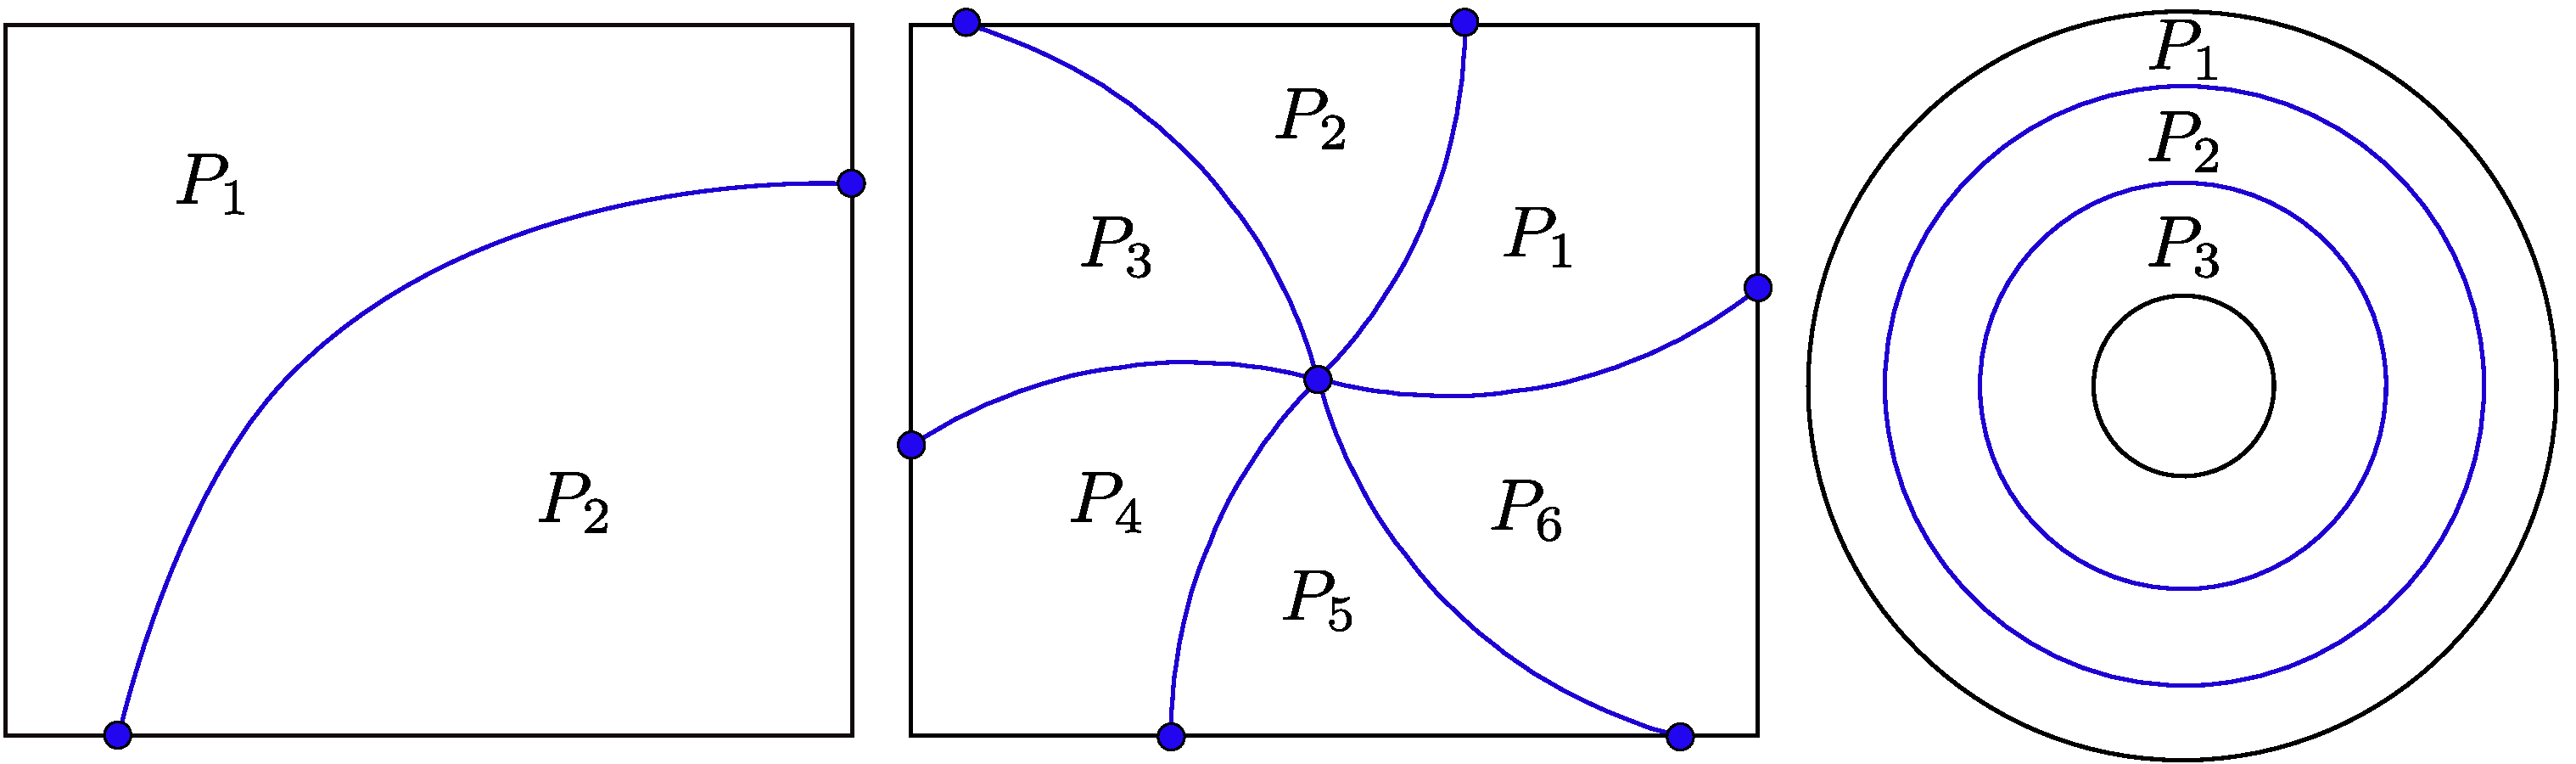
\includegraphics[width=\linewidth]{figures/crease_patterns}
	\caption{Curved crease patterns, decomposing a pattern into multiple components $P_i$ and intersecting at crease vertices. Boundary curves in black, crease curves in blue.}
	\label{fig:crease_pattern}
\end{figure}
We are interested in deformations on curved folded surfaces that keeps them curved folded. Viewed separately on each patch $P_i$, these deformation are $C^2$, though they often introduce tangent discontinuities along the patches intersections. At \cite{demaine_lens} the authors refer to creases that remain $C^2$ as \textit{smoothly folded} creases (though they define it as $C^1$ they prove that this implies that they are $C^2$). In particular we are interested in such continuous deformations, or deformation flows \cite{rabi2018shape}, which we refer to as curved folding flows. We denote these flows by a continuous map $S(t), 0 \leq t \leq 1$, where each $S(t)$ is a curved folded surface and the flow is $C^2$ when limited to each patch. We often look at the case where the starting point $S(0)$ planar. In this paper we focus on modeling isometric curved flows, which we also refer to as \emph{folding}. These flows can can be used to model physical paper or metal folding, though most of our observations and tools can also be used to model curved folding flows that are not isometries. Non-isometric developable deformations can be useful for design tasks where the a-priori flattened shape is unknown \cite{rabi18,rabi2018shape} .

\subsection{Model} \label{sec:model}
We follow the work of \cite{rabi2018shape} by modeling each patch $P_i$ as a discrete orthogonal geodesic net (see \figref{fig:curve_on_dog}). We represent a crease as piecewise linear curves, whose points $c(i)$ are represented by the curves' intersection point with the grid edges. Each point $c(i)$ is a linear combination of two vertices on a DOG: $c(i) = t v_i + (1-t)v_j,$ where $0 \leq t \leq 1$ and $v_i,v_j$ are too neighbour vertices on the grid.  Each point on a crease lies on each of the $m \geq 2$ different patches, essentially duplicated. If $c(i)^1,c(i)^2,....,c(i)^m$ are the representation of $c(i)$ on the different patches, we enforce constrain these duplicated points have equal coordinates (see \figref{fig:curve_on_dog}).
We trivially extend the represntation at \cite{rabi2018shape} to support intersecting curves by adding grid lines at crease vertices (see \figref{fig:piecewise_dog_from_crease} and \figref{fig:curve_on_dog}).

\begin{figure} [h]
	\centering
	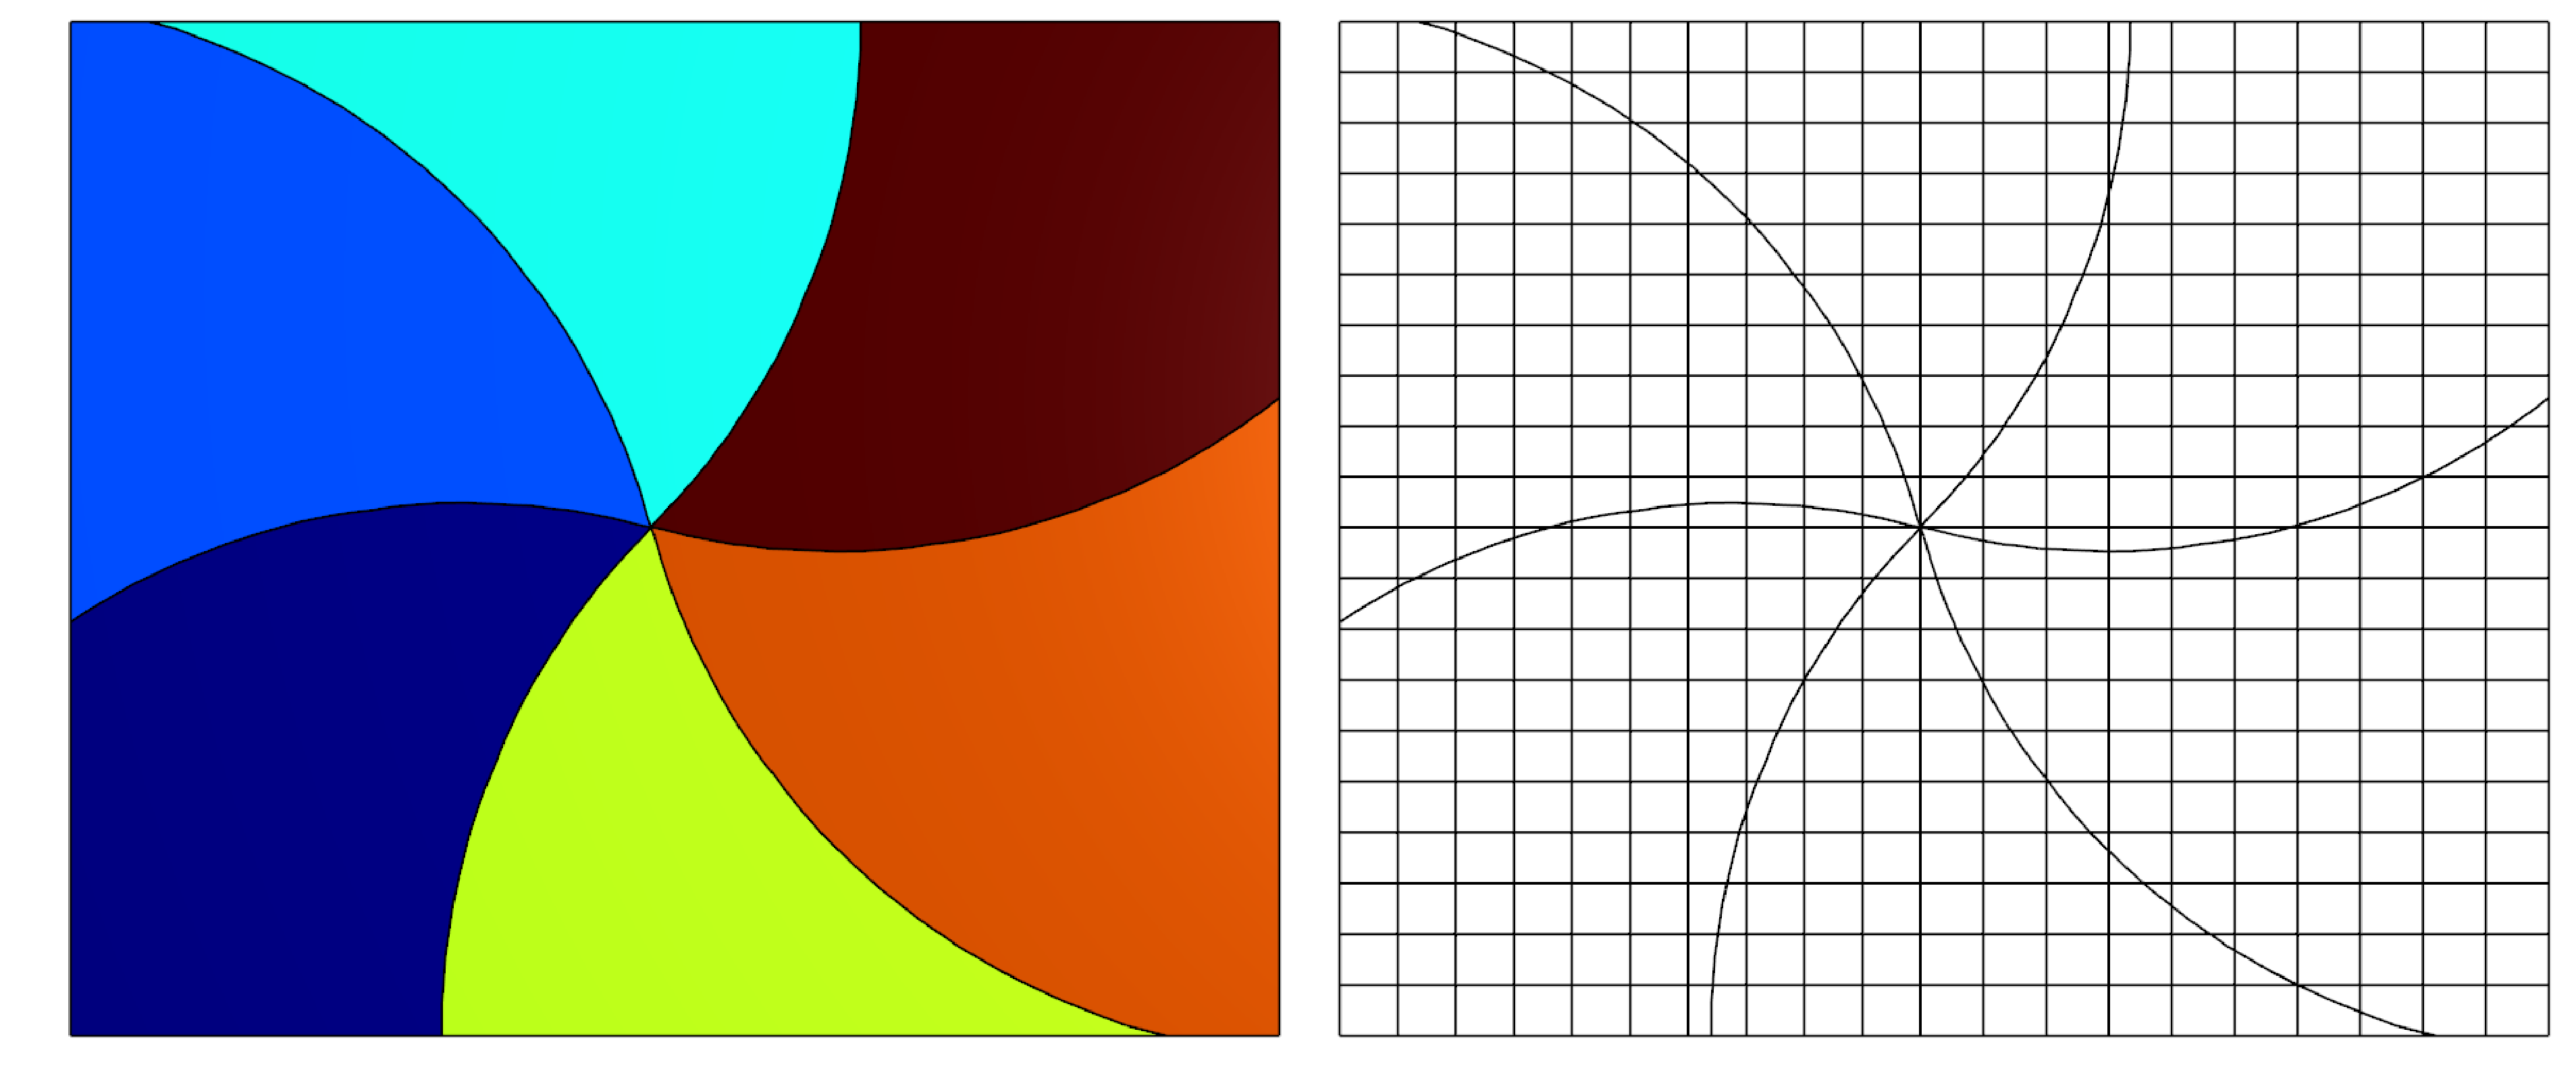
\includegraphics[width=0.8\linewidth]{figures/piecewise_dog_from_crease}
	\caption{Given a crease pattern, we create a DOG for each segment (colored differently), and use the boundary constraints as done in \cite{rabi2018shape}.}
	\label{fig:piecewise_dog_from_crease}
\end{figure}

\begin{figure} [h]
	\centering
	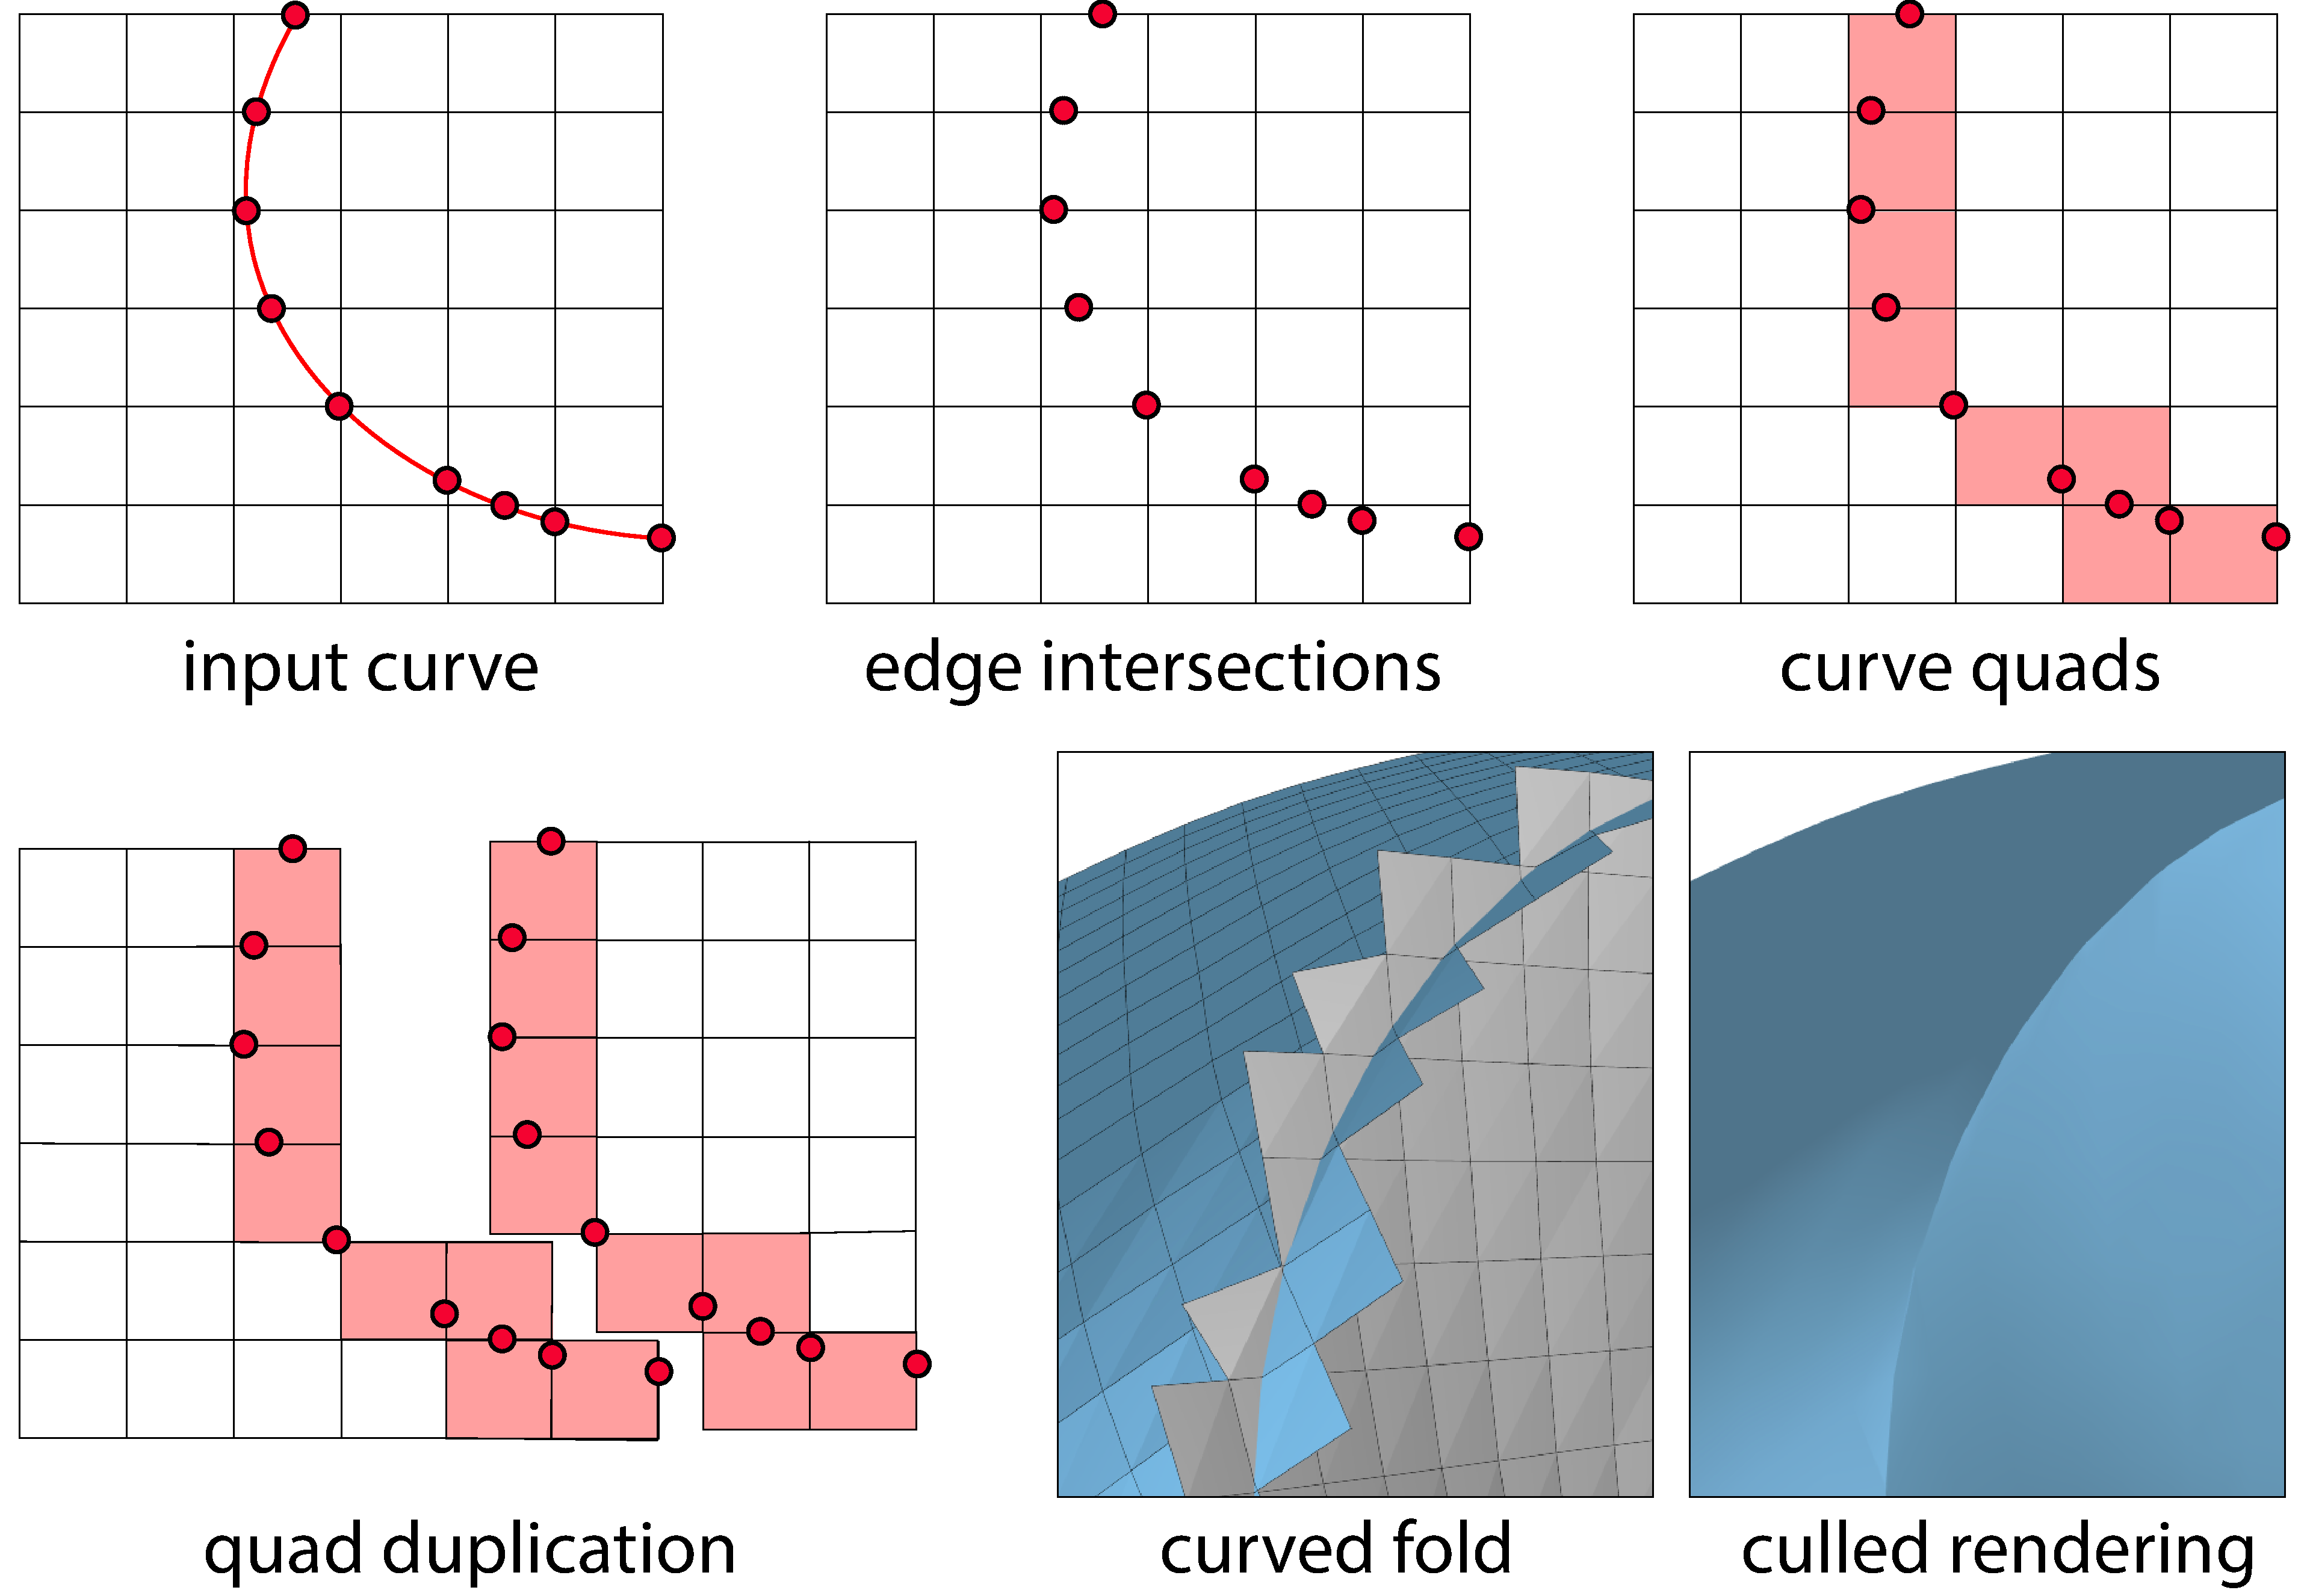
\includegraphics[width=0.8\linewidth]{figures/curve_on_dog}
	\caption{Picture taken from \cite{rabi2018shape}.}
	\label{fig:curve_on_dog}
\end{figure}

\subsection{Desiderata}
Our goal is to develop tools for the exploration of curved folded shapes on top of piecewise DOGs by means of deformations. Our choices are guided by the following ground rules for deforming DOGs:
\begin{enumerate}
  \item Perform homotopy based optimization \label{homotopy_opt}
  \item Minimally constrain DOGs \label{minimal_const}
%  \item Use accurate functionals \label{accurate_func}
%  \item Use simple functionals
\end{enumerate}
\textbf{Homotopy based optimization} is motivated both theoretically and empirically; Modeling DOGs requires solving highly constrained and non linear optimization problems, yet the theory of DOGs guarantees the existence of nearby solutions if one starts at a feasible point. In fact, generally the shape space of DOGs is a smooth manifold \cite{rabi2018shape}. This observation is worthwhile in practice; DOGs exploration was demonstrated to perform well using smooth flow, or homotopy based optimization methods both for handle based editing tasks as well for more complicated deformations such as curve-constraining flows \cite{rabi2018shape}. \\
\textbf{Minimally constrain DOGs.} As DOGs are already heavily constrained, one needs to carefully choose which quantities to constrain by hard constraints, and which ones should be optimized using soft constraints. This is essential to avoid locking, or ill-posed problems in case the constraint gradients are linearly independent \cite{rabi2018shape}. In particular, the rigidity analysis in \cite{rabi18} demonstrates that one cannot fix all edge length exactly, or likewise demand a DOG to also be a Chebyshev net. We note however that this can be done approximately and to a low tolerance as a DOG is a chebyshev at the smooth limit and at the smooth limit there is a rich set of exact isometries. The folding constraints at \secref{sec:folding} where chosen such that they could be satisfied \textit{exactly}, and so that in practice they vanish once the surface is sufficiently folded, just like a piecewise smooth curved folded surface. \\
%\textbf{Accurate functionals.} We look for constraints and objectives that are accurate and as often in the case with DOG objectives, converge under sampling of a smooth orthogonal geodesic net \cite{rabi18,rabi2018shape}. \\
%\textbf{Simple functionals.} We strongly prefer sparser objectives with a lower degree as possible. To that end, we leverage the regularity of the DOG meshing and theory on smooth orthogonal geodesic nets in our derivations. \\